\section{Trend Data for Explainability papers}
\begin{figure}[h]
    \centering
    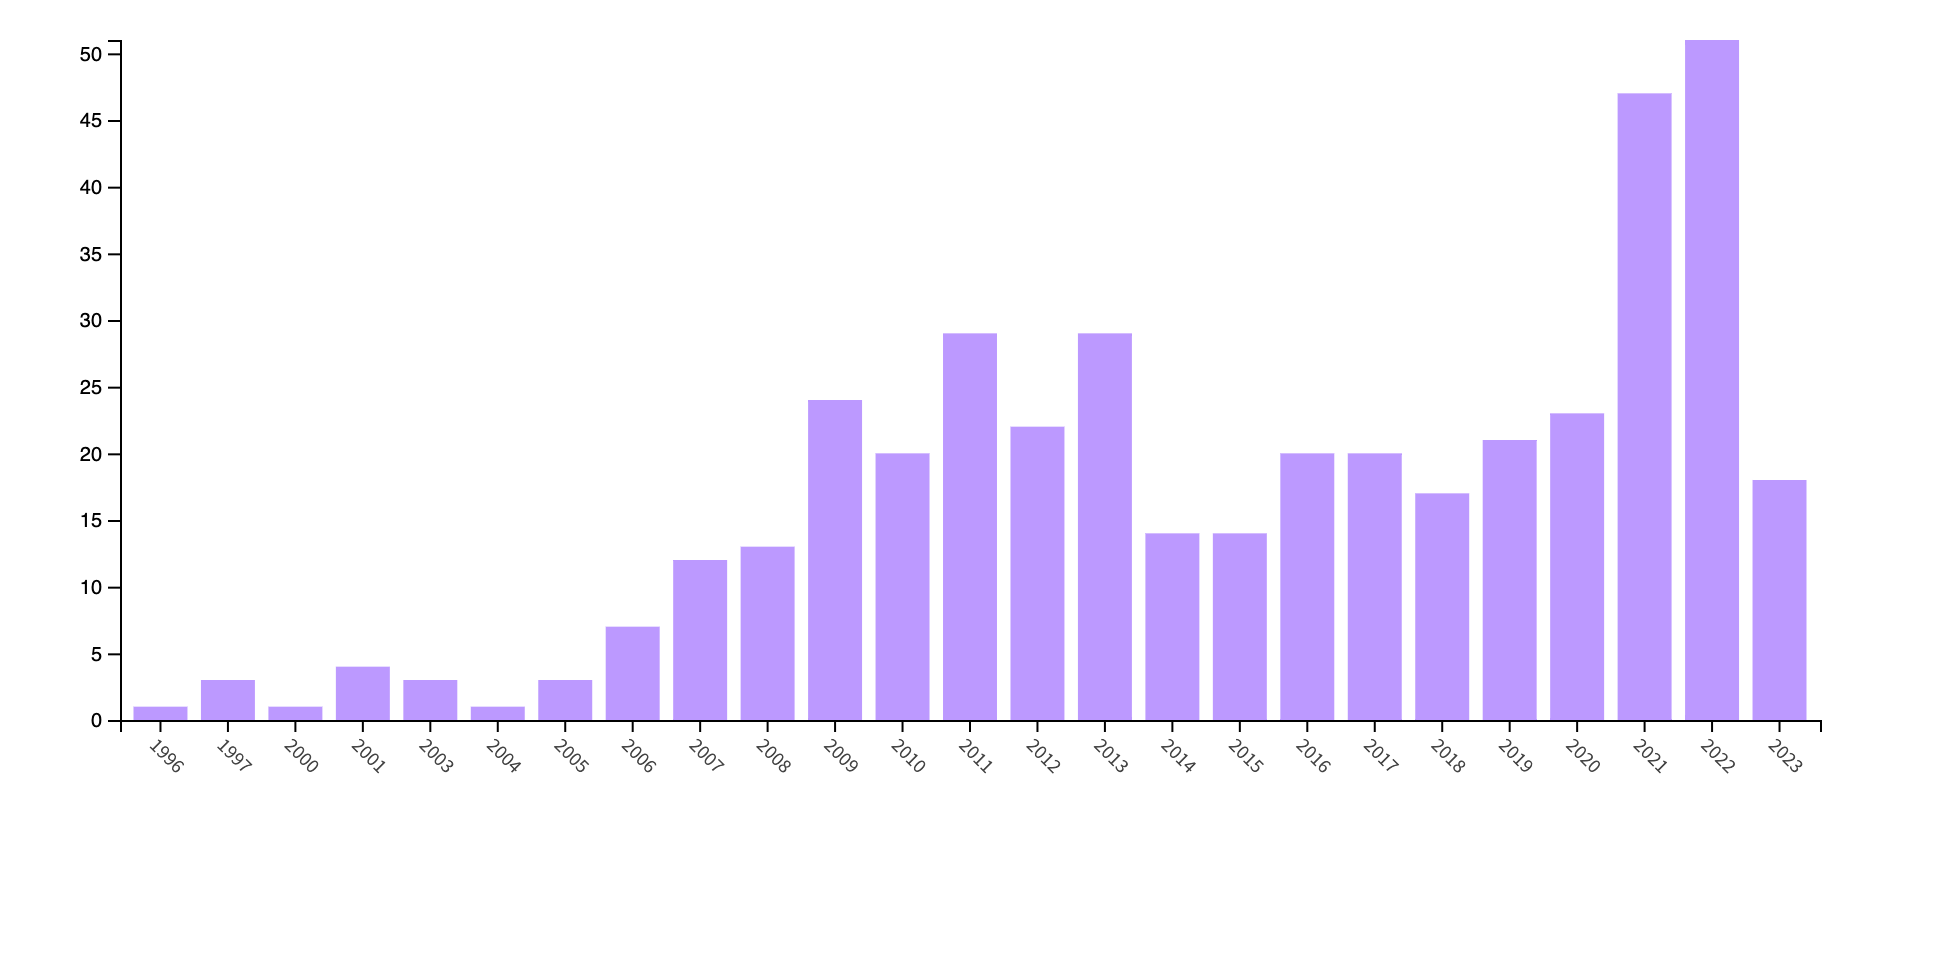
\includegraphics[width=.75\textwidth]{images/publications-keywords.jpg}
    \caption{
    Number of publications published per year with keywords (inclusive OR): explainable, explainability, explainer, interpretable, interpretability. Data and graphic included herein is derived from Clarivate Web of Science. © Copyright Clarivate 2023. All rights reserved.}
    \label{fig:publications-keywords}
\end{figure}

\section{EvolveGCN Temporal Layer Weighting}
\begin{figure}[h]
    \centering
    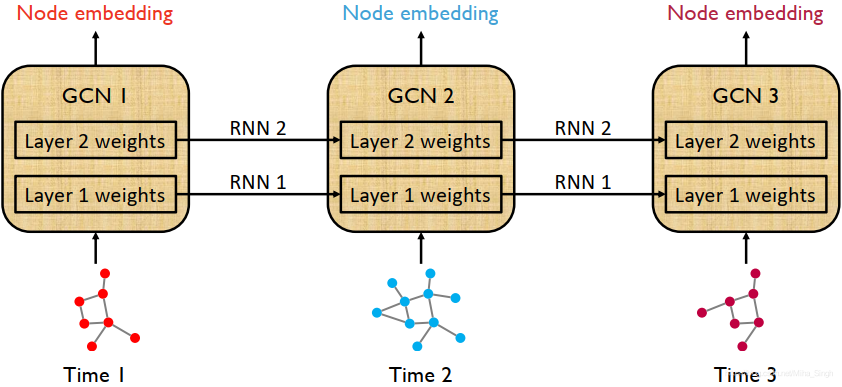
\includegraphics[width=.75\textwidth]{images/evolve-gcn.png}
    \caption{Layer parameters are evolved over time via RNN\cite{pareja_evolvegcn_2019}. Each snapshot has its own GCN. Temporal information is used to upgrade the weights matrix.}
    \label{fig:EvolveGCN}
\end{figure}

\section{Table 3. GNN Prediction and Explanation in Dynamic Graphs}
\begin{sidewaystable}
    \centering
    \begin{tabular}{|l|l|l|l|l|l|l|l|l|}
        \hline
        Paper & Year & Technique & Technique class & Explanation & Black Box & Task* & Graph & Application \\ \hline
        Ye et al.\cite{ye_explainable_2023} & 2023 & BrainNetX & Gradient(SA) & Node & STpGCN & NC & Temporal & brain \\
        He et al.\cite{he_explainer_2022} & 2022 & TGNNExplainer & Surrogate(PGM) & Subgraph & TGNN & NOP & Temporal & traffic \\
        Limeros et al.\cite{limeros_towards_2022} & 2022 & XHGP & Perturbation(counterfactual) & Interaction & GAT-GRU & MP & Temporal & autonomous cars \\
        Xie et al.\cite{xie_explaining_2022} & 2022 & DGExplainer & Decomposition(LRP) & Features & GCN-GRU & NR & Dynamic & traffic \\
        Fan et al.\cite{fan_gcn-se_2021} & 2022 & Interpretability & Attention & Snapshot & GCN-SE & NC & Dynamic & bibliography \\
        Yao et al.\cite{yao_interpretable_2021} & 2021 & Interpretability & Decay rate & Edge & RNN-GCN & NC & Edge Dynamic& bibliography \\
        Yang et al.\cite{yang_fraudmemory_2019} & 2019 & Interpretability & Sub Scores & Time & FraudMemory & NC & Edge Dynamic & Fraud \\
        \hline
    \end{tabular}
    *NC= node classification, NOP= node output prediction, NR=node regression, MP=motion prediction
    \label{table-3-full}
\end{sidewaystable}
